\documentclass[a4paper]{article}
\usepackage{amsmath}
\usepackage{amsfonts}
\usepackage{mathtools}
\usepackage{amsthm}
\usepackage{amssymb}
\usepackage{listings}
\usepackage{graphicx}

\begin{document}
\begin{titlepage}
  \begin{center}
    Title: Pandemic Modeling and Simulation \\
    Course: Modeling and Simulation \\
    Author: Jeffrey Ahn \\
  \end{center}
\end{titlepage}

\newpage

\begin{center}
\textbf{1. Introduction}
\end{center}

Towards the end of
December 2019, a cluster of cases related to pneumonia were reported in
Wuhan, China. By early February 2020, China recorded 811 deaths surpassing the 2003 SARS
epidemic. On March 11, 2020, the World Health Organization (WHO) declared the
growing outbreak a pandemic as cases of COVID-19 are reported all over the
globe. At the time of this writing the author and his fellow students and
colleagues are told by the state and federal government to exhibit ``social 
distancing"--a self imposed quarantine to reduce the spread of the disease. This 
pandemic will no doubt be the defining calamity of the year.

The ultimate goal of this project is to build a model valid enough to be used
to simulate any epidemic or pandemic event. The model can then be 
used to predict growth and possibly reduce the spread of diseases in an
epidemic.

\begin{center}
  \textbf{2. Background}
\end{center}

This pandemic model is based primarily on epidemiological science. In the model,
an arbitrary disease is spread within and through neighboring populations to
individuals. This is to simulate the spread of COVID-19
by contact via respiratory droplets (e.g. sneezing and coughing) or through touching a 
contaminated surface and then
their face (however, the latter is not thought to be the primary way the virus spreads).
This information is provided directly from the Center for Disease Control (CDC). 

Other epidemiological factors include how contagious the virus is which 
directly effects the infection rate. Some viruses are more
contagious than others (e.g. measles is highly contagious). It is not currently
known exactly how contagious SARS-CoV-2 (the specific strain responsible for COVID-19)
really is, but it is presumed that it is most contagious when the disease
carrier is symptomatic (i.e. the disease is in full swing). It is hypothesized by 
epidemiologists that the reason what makes COVID-19 a good candidate for a pandemic is 
its incubation period. A longer incubation period makes it difficult to
determine if a person is a carrier for the disease without a testing kit (which
are very limited) and until the carrier becomes symptomatic, he/she will likely
have spread the disease to others.

Another factor to consider that 
is mobility. Indeed, the rate at which a disease spreads to other regions
in a city, state, country etc. (i.e. at a ) is influenced by the spatial 
and mobile patterns within the region. Had the virus been contracted in a low
population, rural village with little to no transportation in and out, the
disease would likely have converged (flattened-out) long ago with only a few 
and local casualities. Then imagine the same disease being released to a handful
of people at an international airport and the difference is the latter case
results in an epidemic. The mobility patterns can be estimated by looking at the
population distribution grid of Wuhan and imposing this data on a map of the
Wuhan Metro transit system. This can be used a rough approximation of intercity
mobility.

\begin{center}
  \textbf{3. Model Development}
\end{center}

The first draft of this model I tried to map data from various online sources the
population density and public transportation lines onto a Google map and then tried
to construct ``flow" between two latitudinal and longitudinal coordinates. While
the mapping of the public transportation lines was successful, finding an
accurate database of population densities by lat/long coordinates was not and
the tools were complicated and difficult to use. 

A different approach was to simulate a single population as a 2-dimensional grid
of cells where each cell has a sub-population. The sub-populations then simulate
the spread of the disease within their own cell and then next the model simulates
the spread of the disease to other surrounding cells. This model was simple
enough to code in Python and robust enough to produce accurate real-world
results. The data needed to create the model could be extracted from
interpolating points from www.worldometer.info/coronavirus.com which tracks data
about COVID-19 at a global scale. Things like infection rate and incubation
period could be estimated using these numbers. Exact specifications of the model will
be discussed in greater detail in following sections.

\begin{center}
  \textbf{4. Model Description}
\end{center}

The model is a continuous one which makes equations and assumptions about aggregated 
populations and is simulated in regular time steps (days). As mentioned above, it starts with 
a 2D grid of cells. In each cell contains a scalar value representing the cell's
sub-population. Each sub-population is subdivided into three mutually exclusive
categories: 1. Susceptible (not Infected), 2. Infected, 3. Removed (either
recovered from infection or dead). Keep in mind that for any cell at any
point in time must be zero-sum i.e. Susceptible + Infected + Removed = size of
sub-population. Every cell in the grid starts off with only Susceptible
state populations. The way the size of each sub-population was distributed for each cell was
by imposing a 2D Gaussian curve over the grid. The height at each cell
of the Gaussian represents the proportion of the global expected population (arbitrarily
set to 1,000,000) size for that cell. Multiplying each cell by this expected population then 
gives the actual sub-population size for that cell.

\begin{figure}[ht]
  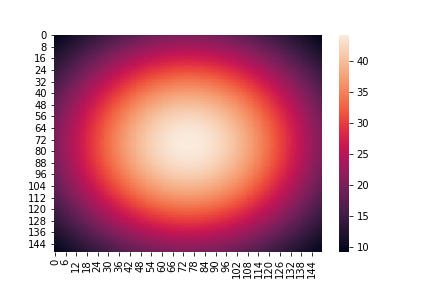
\includegraphics[scale=0.4]{../population_dist.png}
  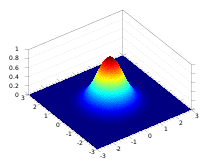
\includegraphics[scale=0.7]{../2dgauss.png}
  \centering
  \caption{(a) The actual heatmap created by matplotlib in the simulation 
    which is a Gaussian distribution over a 150 by 150 grid. The higher intensities
  in the center implies larger sub-population ($> 40$ people). (b) A picture of
2D Gaussian for reference. The larger spread in (a) is done by increasing the
standard deviation. }
\end{figure}

Next step was to introduce Infected cells into the population. Two cells were chosen
randomly to be infected ones. The proportion of Infected was also chosen
randomly. Once chosen, the number of Susceptibles in these cells had to be
appropriately deducted to maintain zero-sum rule.

\begin{figure}[ht]
  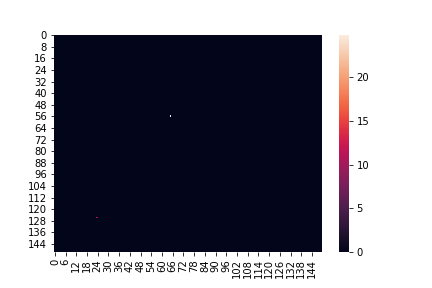
\includegraphics[scale=0.70]{../infected_cells.png}
  \centering
  \caption{Two Infected cells in a separate Infected grid. Note that all other cells are black meaning there
  are no other Infected cells in the initial state.}
\end{figure}

After the infected cells were chosen, the model would simulate a single day by starting
from an Infected cell (once a cell has more than 1 infected it counts as an
infected cell) and ``spreading'' its infection to other random cells which
were chosen by a random Gaussian process (cells closest to it were more likely
to be infected than the ones further away). This was done for every cell that
contained a non-zero infected population. After that, each cell was to undergo
its own self-contained intracell (intra = within) infection process where Susceptible were converted to
Infected and Infected were converted to Removed. 

The procedure would be repeated until no Susceptibles remained or within a
finite (10-40 days depending on the constraints, more on this later) whichever came first.

\newpage

\begin{center}
  \textbf{5. Verification and Validation}
\end{center}

Now that a high-level overview of the model has been explained, we dive deeper
into the details of the model. We discuss two important modeling choices: How
intracell infection step is modeled and second how the intercell spreading step is
simulated.
\bigskip

\textbf{Intracell Spreading}

Within each sub-population, Susceptibles are converted to Infected and then to
Removed states. The rate at which these occur can be modeled using differential
equations. Indeed, in 1927 A.G. McKendrick and W.O. Kermack developed the
Kermack-McKendrick theory which gave rise to the SIR (Susceptible, Infected,
Removed) model that predicts the distribution of infectious disease over time.
The SIR model is used in this project for the intracell spreading step.

Let $S(t), I(t), R(t)$ be the number of susceptibles, infected, and removed at a 
given time $t$ respectively and let $N$ be the sum of the three (always
constant). Let $\beta$ be transmission rate per person per unit time then we
have our first differential equation, the Susceptible Equation:

\begin{equation}
  \frac{dS}{dt} = -\beta I(t) \frac{S(t)}{N}
\end{equation}

This says that the rate that susceptibles are converted to infected is related
by the total number of infected times the transmission rate times the proportion
of susceptibles. Assuming a purely heterogeneous population, an
infected person comes into contact with a susceptible with probability
$\frac{S(t)}{N}$, then eq (1) describes the expected number of new infected
individuals at time $t$ which is equal to the rate at which $S(t)$ declines.

Next let $\gamma$ be the recovery rate per person per unit time. Then the
Infected Equation is as follows:

\begin{equation}
  \frac{dI}{dt} = \beta I(t) \frac{S(t)}{N} - \gamma I(t)
\end{equation}

The first term in this equation describes the rate at which new infected are
accumulating (which is exactly the negative of eq (1)). The second term
describes the rate that infected are being removed (recovered or dead) which
is the rate of recovery per person, $\gamma$ times $I(t)$ the total number of
infected. This equation is an example of inflow - outflow.

Lastly, we have the Recovery/Removed Equation: 

\begin{equation}
  \frac{dR}{dt} = \gamma I(t)
\end{equation}

Which says the rate of recovery is equal to the rate individuals are being
converted from infected to removed (the last term in eq (2)).

It is helpful to think of each of the equations with a flow diagram. Imagine
three cylinders stacked on top of each other, Susceptible, Infected, and Removed
respectively with water (uninfected people) contained only in the Susceptible cylinder 
at the start. Then a spout from S is opened and pours into I and a spout in I is opened
which pours into R. The SIR equations describe the rate at which these spouts allow 
water to flow into each cylinder.

So for each ``day'' event in the simulation, these set of equations would be
used to calculate the change in each of the three quantities for each sub-population 
by using Euler's method of integration and letting $\Delta t=1$. In the simulation the
three values for S, I, and R are stored in three separate grids and for any cell
${(i,j)}$, $S_{i,j} + I_{i,j} + R_{i,j} = N_{i,j}$ where $N_{i,j}$ is the total
size of the sub-population.


The following will explain how this model determined the constant values of 
$\beta$ and $\gamma$. In the study of epidemiology, $R_0$ is the expected number 
of people in a susceptible population that a single infected person will spread 
the disease over the entire course of their infection. It is modeled formally by 
the following equation:

\begin{equation}
  R_0 = \frac{\beta}{\gamma}
\end{equation}
Where $\beta$ and $\gamma$ are the daily transmission rates and recovery rates
respectively. Note that if $R_0$ is less than or equal to one, the disease remains endemic
(restricted at a controllable level) and for values greater than one, the
disease can be become epidemic. The value of $R_0$ was taken from various
sources online which is estimated to be anywhere between 1.9 - 4.0 (taking the
upper bound of 4 for this simulation but of course can be changed for different runs). 
The value for $\gamma$ can be estimated by taking the reciprocal of the mean
infection duration. If $t_r$ is the mean infection period of a disease in days,
then $t_r^{-1} = \gamma$ is the average rate of recovery which is why in eq (3),
$\gamma I(t)(\Delta t:=1)$ equals the total number of people recovered on day $t$.
The mean infection period of COVID-19 was taken from various sources and estimated to 
be around 9 days. Knowing these two parameters, $\beta$ was solved for using eq (4) and estimated to be around $\frac{4}{9}$ which
can be interpreted as every 9 infected people infects 4 susceptible people every
day.

\bigskip

\textbf{Intercell Spreading}

As discussed in section 4, before intracell spreading occurs, an intercell
spreading phase happens (intercell meaning between two different cells).
One of the two ways this model simulates the spreading of a disease to different locations
(cells) is by using a stochastic process. It was stated earlier that each cell 
randomly chose neighboring cells using a 2D Gaussian distribution centered at itself 
and this is all there is to it. Every cell chooses a list of 8 neighbors to be 
its intercell target for the remainder of the simulation. The number 8 was 
chosen because a cell can technically have at most 8 neighbors (north, east, 
south, west, and the inbetweens). 2D Gaussian was chosen because it reflects how 
people in a city tend to move/travel closer distances with higher probability than further 
distances.

\begin{figure}[ht]
  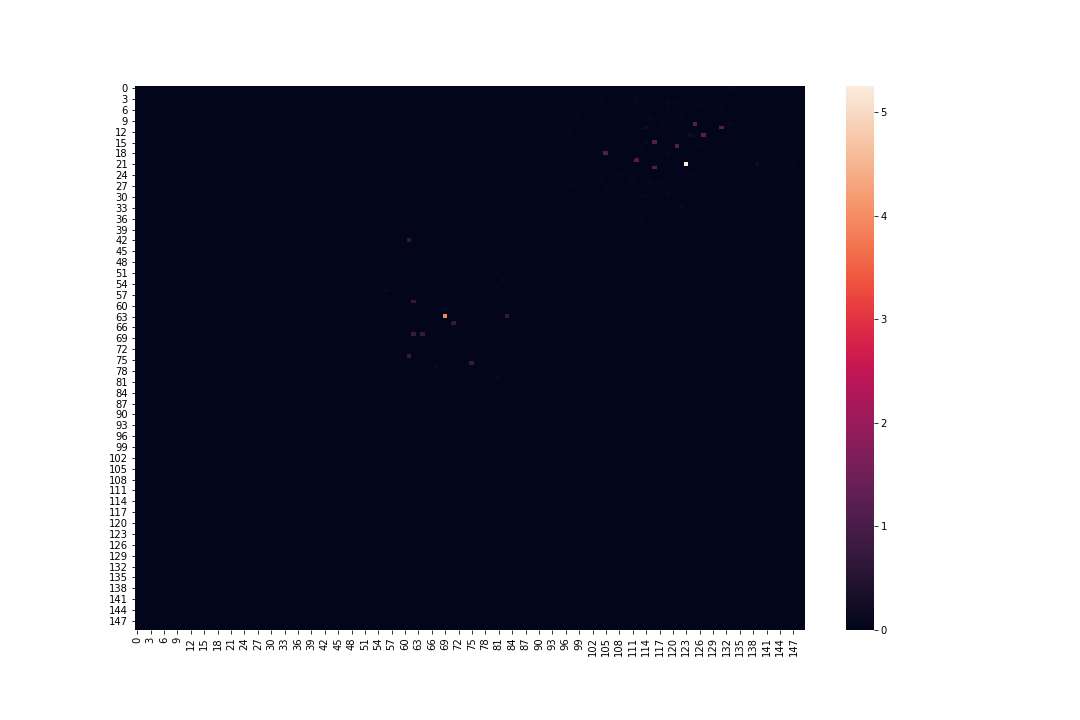
\includegraphics[scale=0.25]{../gaussian_spread/gaussian_spread_1.png}
  \centering
  \caption{Gaussian intercell spreading. Notice the clusters spreading randomly from
  the initial points}
\end{figure}

The other intercell spreading simulation technique used is a well-known algorithm 
in computer science called breadth-first search (BFS). Starting from the initial
(randomly chosen) infected cells, each infected cell targets its 8 most
immediate neighboring cells. The number of new infection is simulated by applying eq
(1) where $I(t)$ is taken from the center cell and $\frac{S(t)}{N}$ are the neighboring
cells. The newly infected cells are put into a queue data structure and the procedure is
repeated until all cells in the grid have been visited. The effect has one that
looks like the disease is gradually emananting from a source. The reason this
method was chosen as an alternative was to simulate the effects of a
stay-at-home quarantine which is imposed almost globally during the COVID-19
pandemic. We will see in greater detail in the next section how effectively a
quarantine can reduce the spread of disease.

\begin{figure}[ht]
  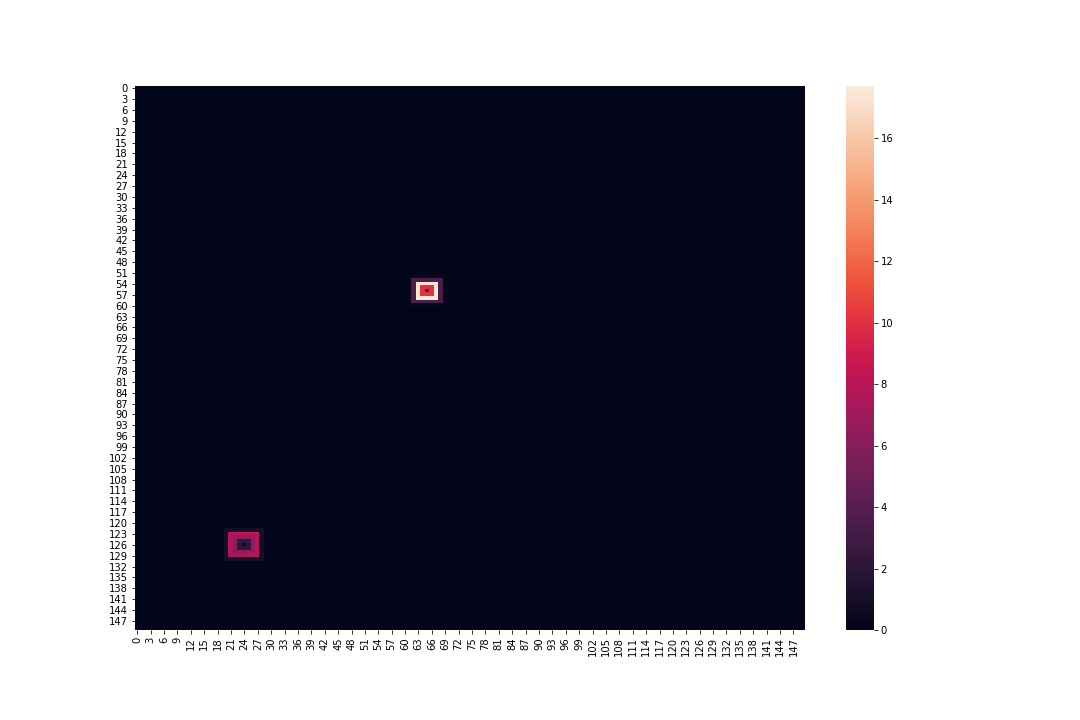
\includegraphics[scale=0.25]{../no_quarantine/no_quarantine_heatmap_3.png}
  \centering
  \caption{Breadth-First Search intercell spreading. Notice the more uniform
  spreading of the infection from the sources.}
\end{figure}

\begin{center}
  \textbf{6. Model Application and Transition}
\end{center}

Both the Gaussian and BFS models were simulated using Python. Recall, the
Gaussian simulation represents a more liberal mobililty pattern than the rigid BFS simulation.
Therefore, the Gauss and BFS models can be thought of as a non-quarantine and quarantine
simulation respectively. But to better simulate a quarantine effect, the values
of $\beta$ (transmission rate per infected person per day) is reduced for the BFS
model to $\beta = \frac{2}{9}$ (half of the previous value) to model a slower daily 
person-to-person contact rate during a quarantine (i.e. ``social distancing'').

\begin{figure}[ht]
  \caption{Simulating with Gaussian spreading. Each image was saved at the end
  of every 5th day in a 40 day simulation. Notice in the last two images, the
once bright areas become dark again, this is because the sub-populations in those 
cells are recovering.}
  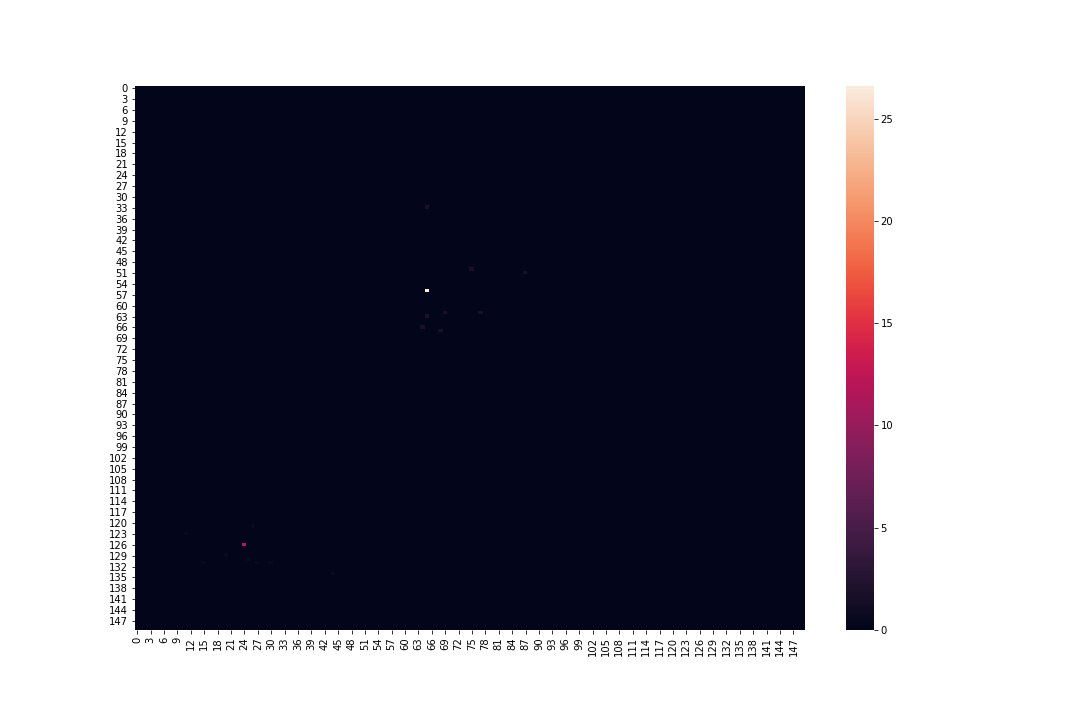
\includegraphics[scale=0.14]{../gaussian_spread/gaussian_spread_0.png}
  \centering
  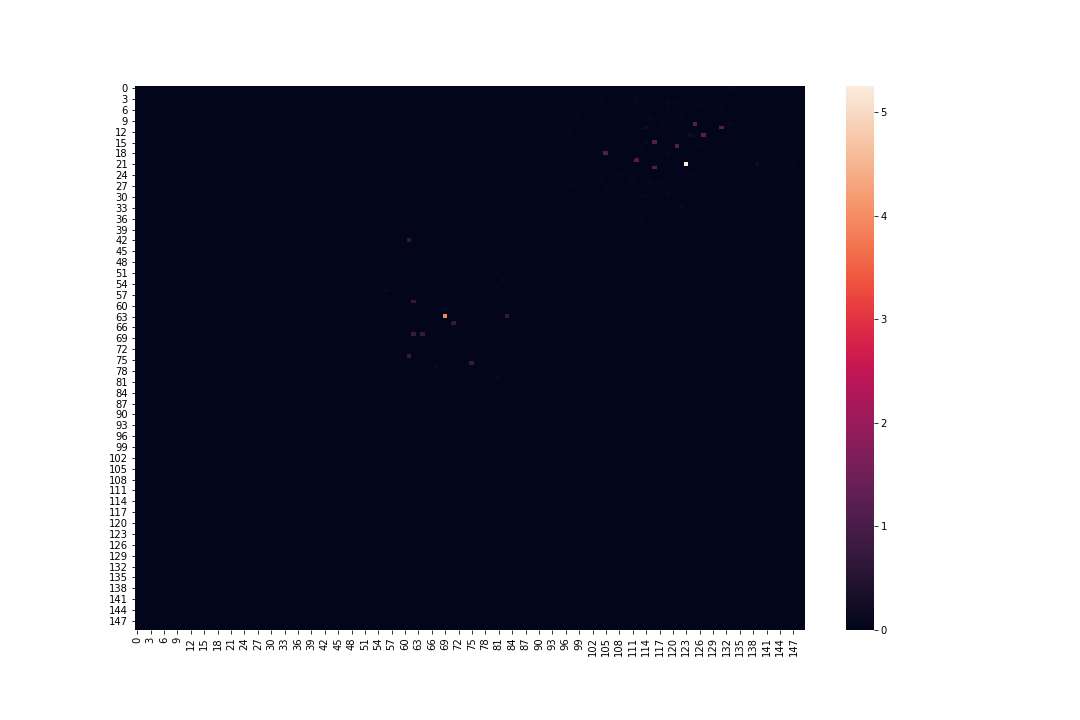
\includegraphics[scale=0.14]{../gaussian_spread/gaussian_spread_1.png}
  \centering
  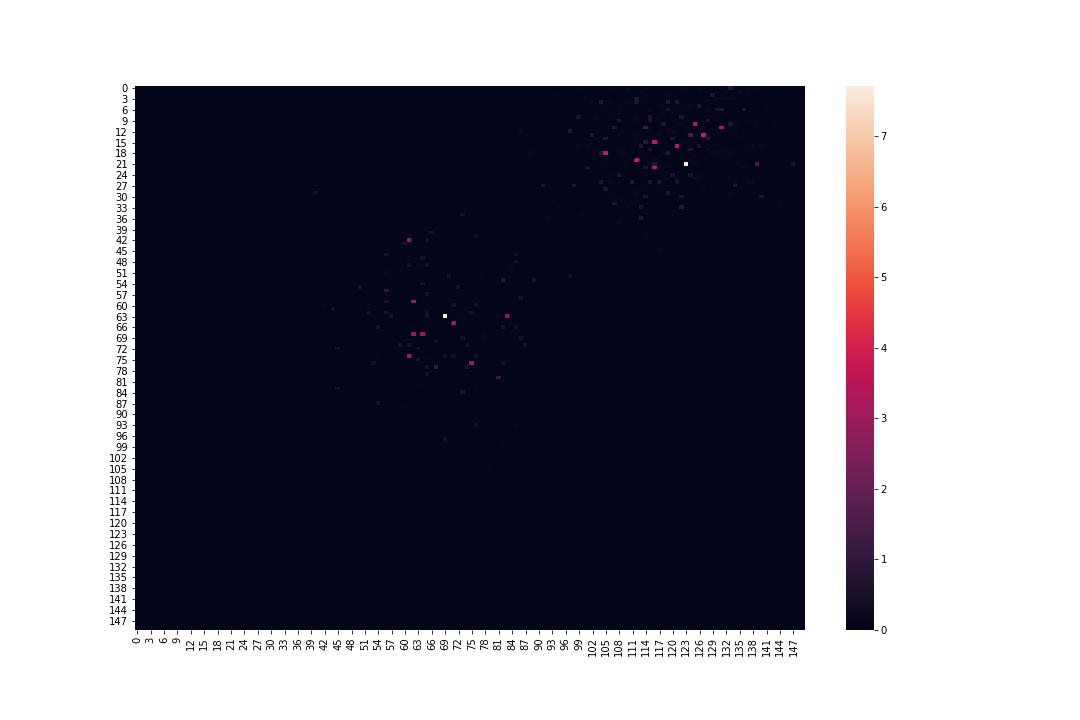
\includegraphics[scale=0.14]{../gaussian_spread/gaussian_spread_2.png}
  \centering
  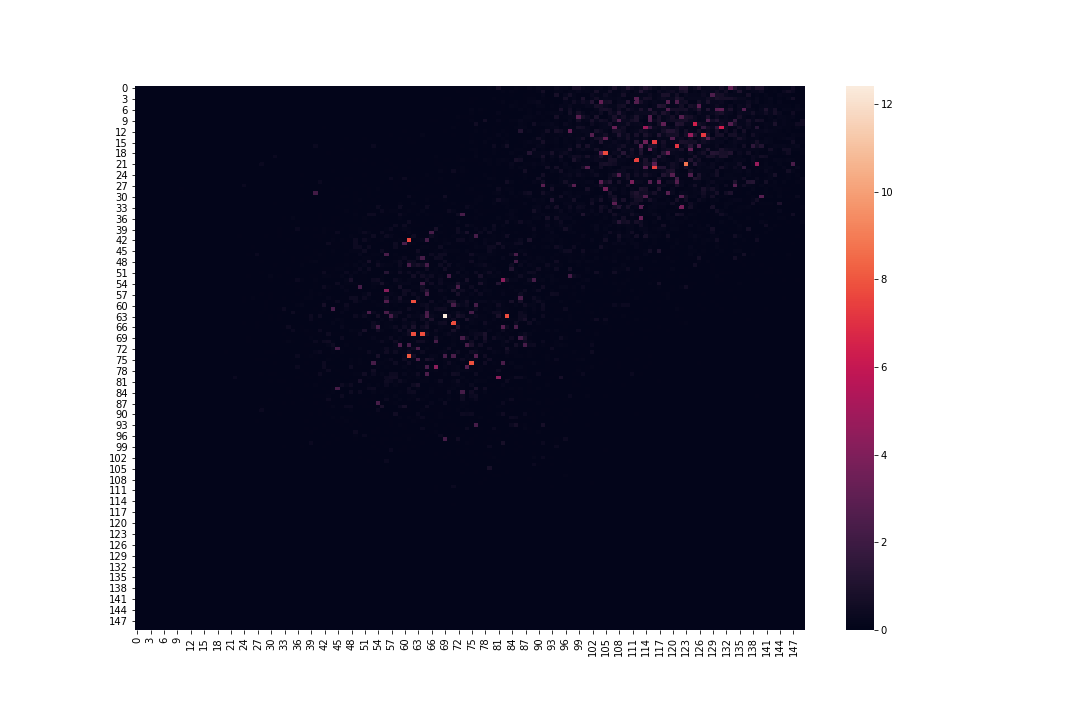
\includegraphics[scale=0.14]{../gaussian_spread/gaussian_spread_3.png}
  \centering
  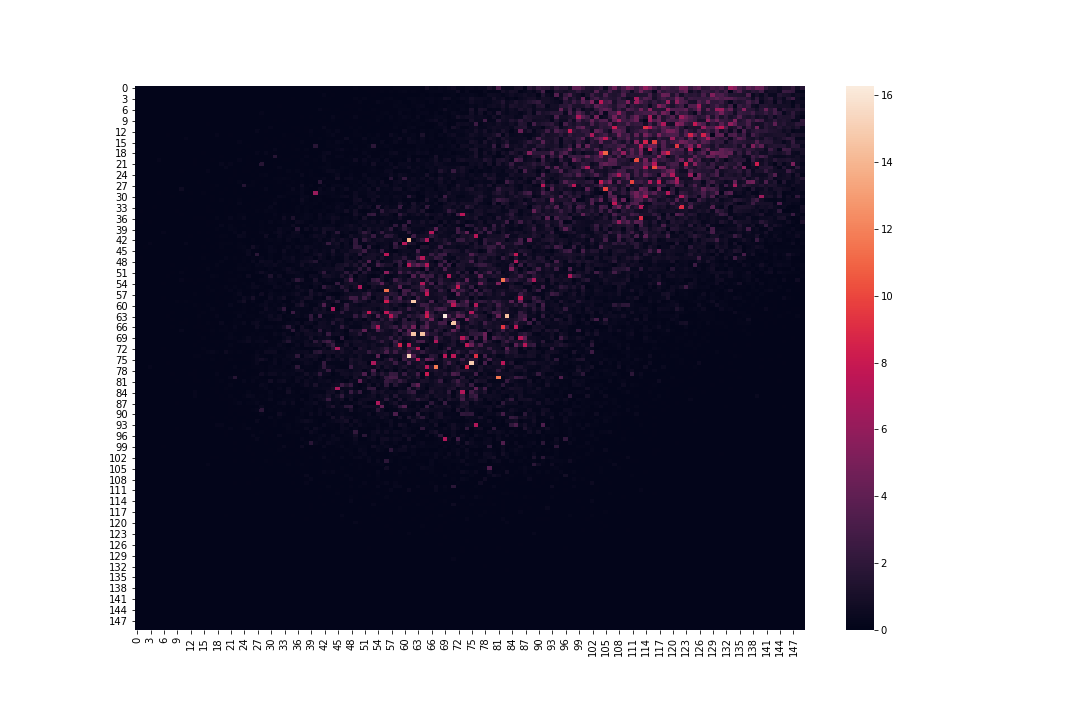
\includegraphics[scale=0.14]{../gaussian_spread/gaussian_spread_4.png}
  \centering
  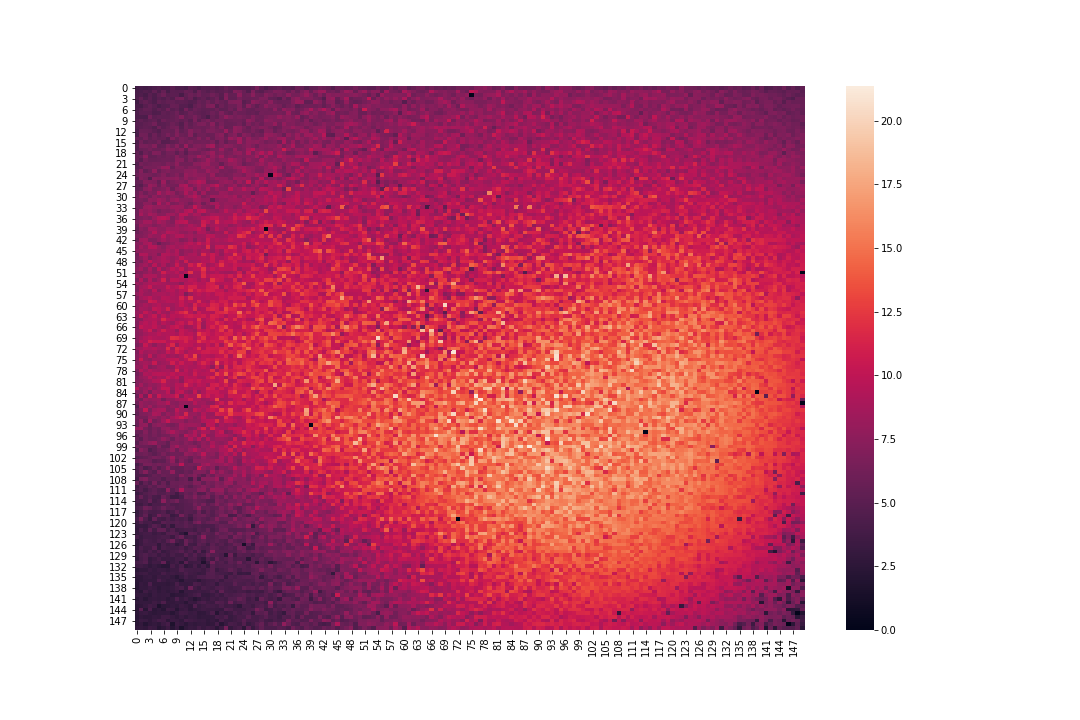
\includegraphics[scale=0.14]{../gaussian_spread/gaussian_spread_5.png}
  \centering
  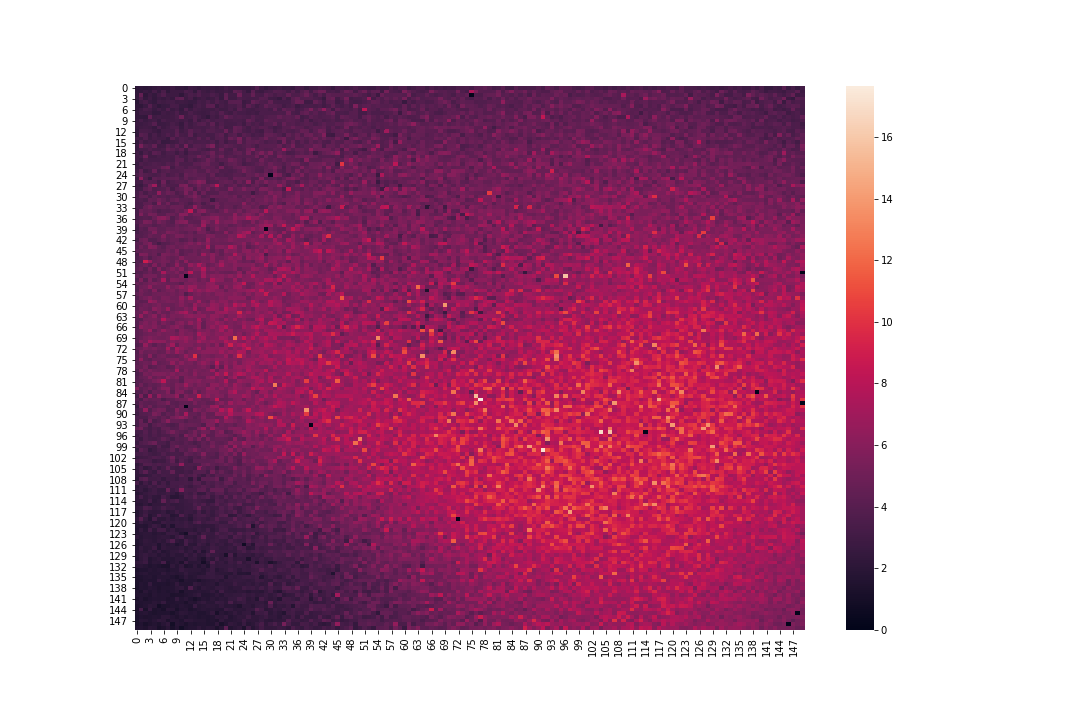
\includegraphics[scale=0.14]{../gaussian_spread/gaussian_spread_6.png}
  \centering
  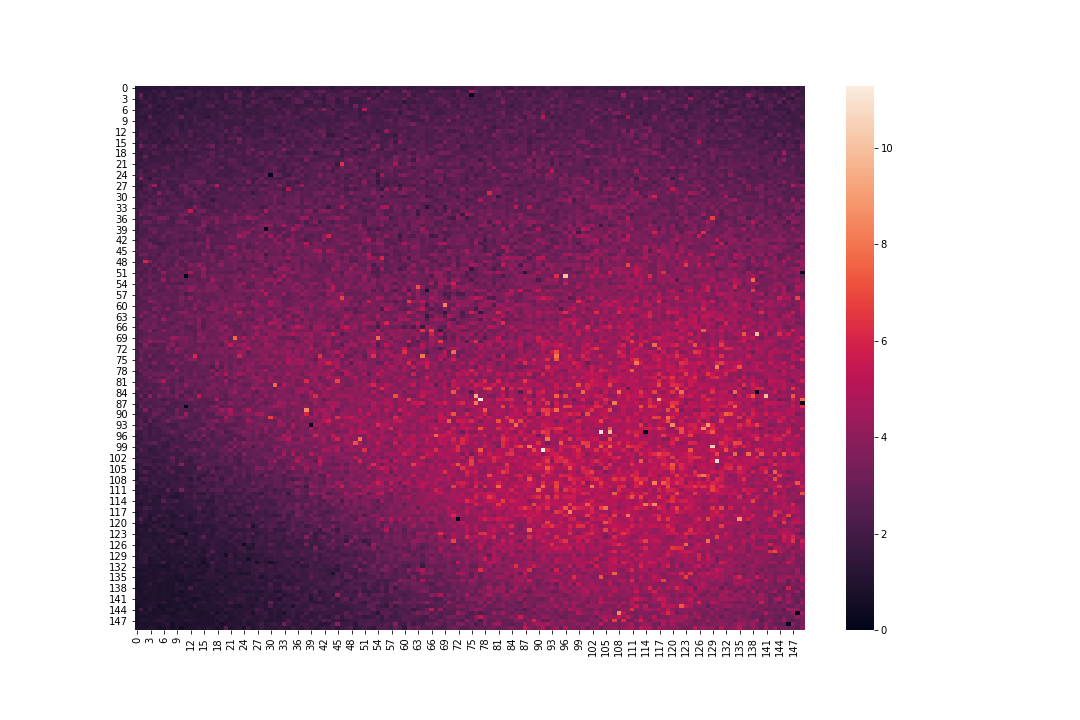
\includegraphics[scale=0.14]{../gaussian_spread/gaussian_spread_7.png}
  \centering
  \centering
\end{figure}

\begin{figure}[ht]
  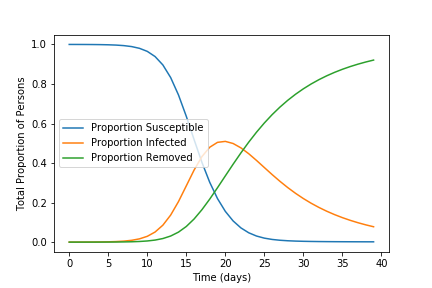
\includegraphics[scale=0.75]{../gaussian_spread/gauss_plot.png}
  \centering
  \caption{Gaussian spread. The plot of proportions of S, I, R over a 40 day
  period.}
  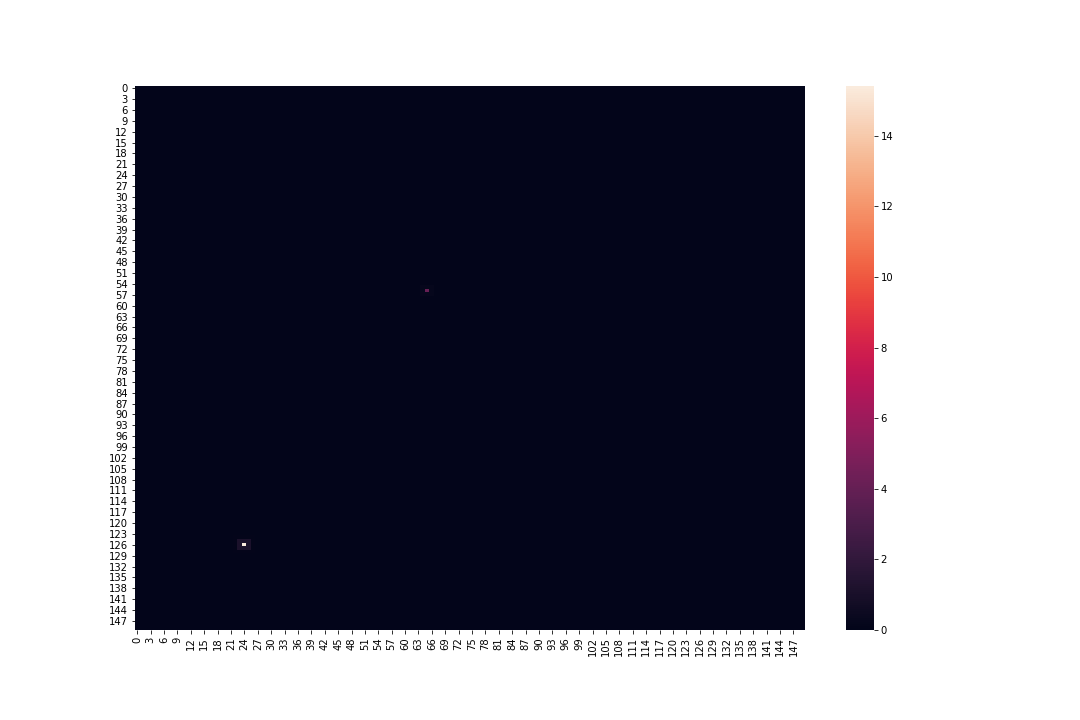
\includegraphics[scale=0.15]{../no_quarantine/no_quarantine_heatmap_0.png}
  \centering
  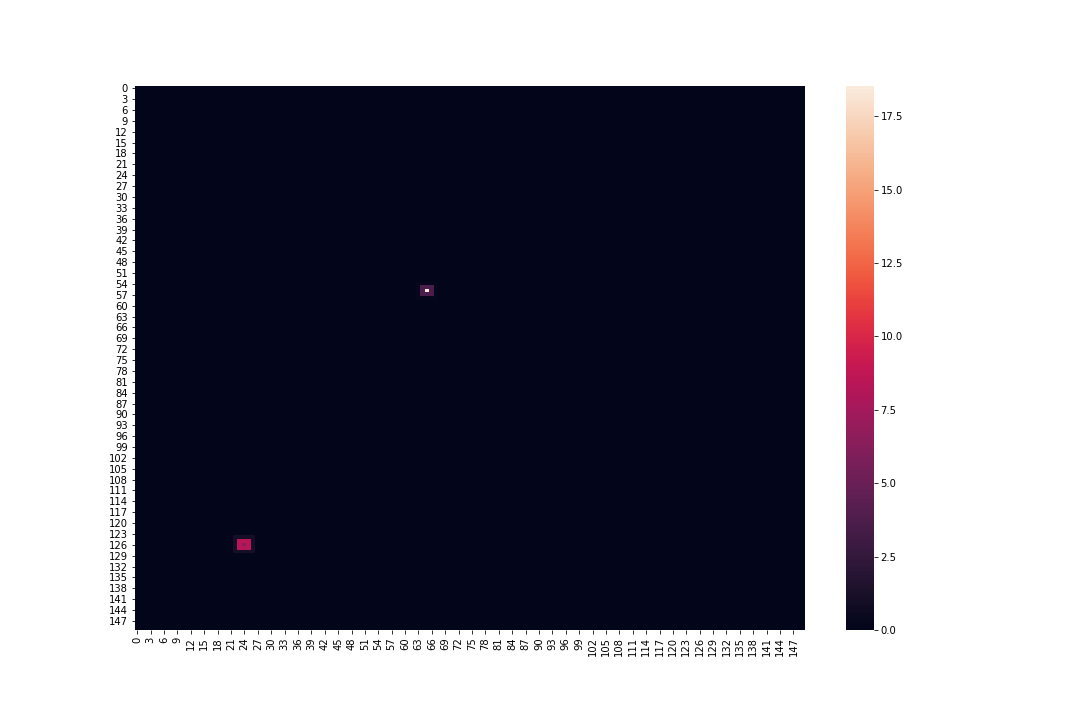
\includegraphics[scale=0.15]{../no_quarantine/no_quarantine_heatmap_1.png}
  \centering
  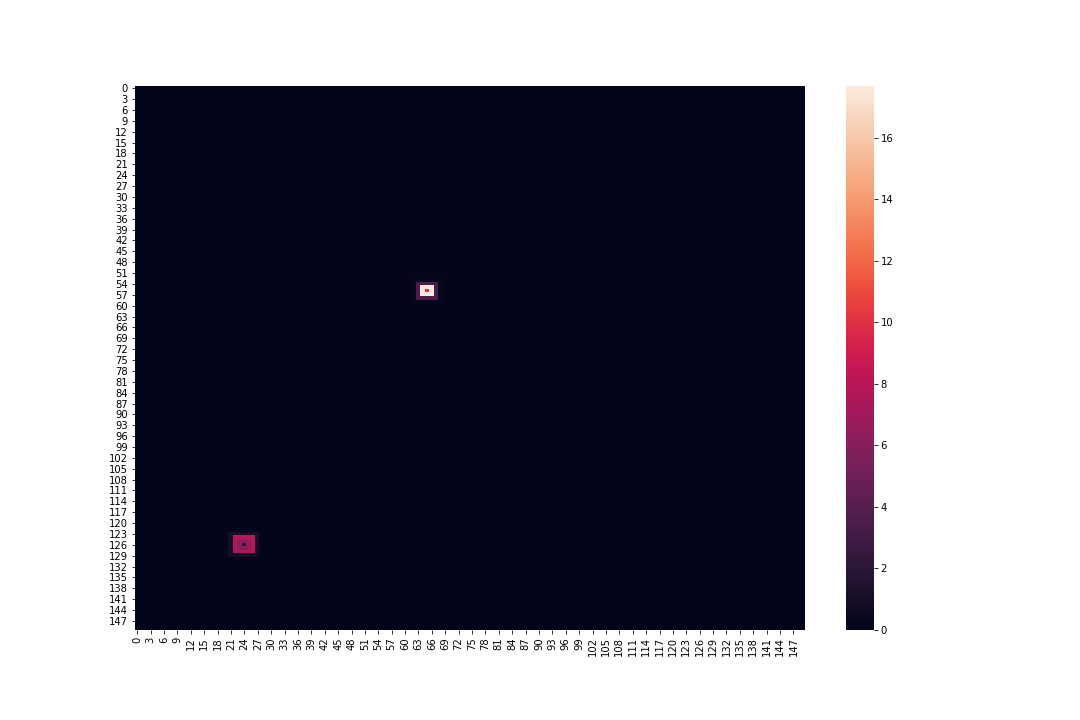
\includegraphics[scale=0.15]{../no_quarantine/no_quarantine_heatmap_2.png}
  \centering
  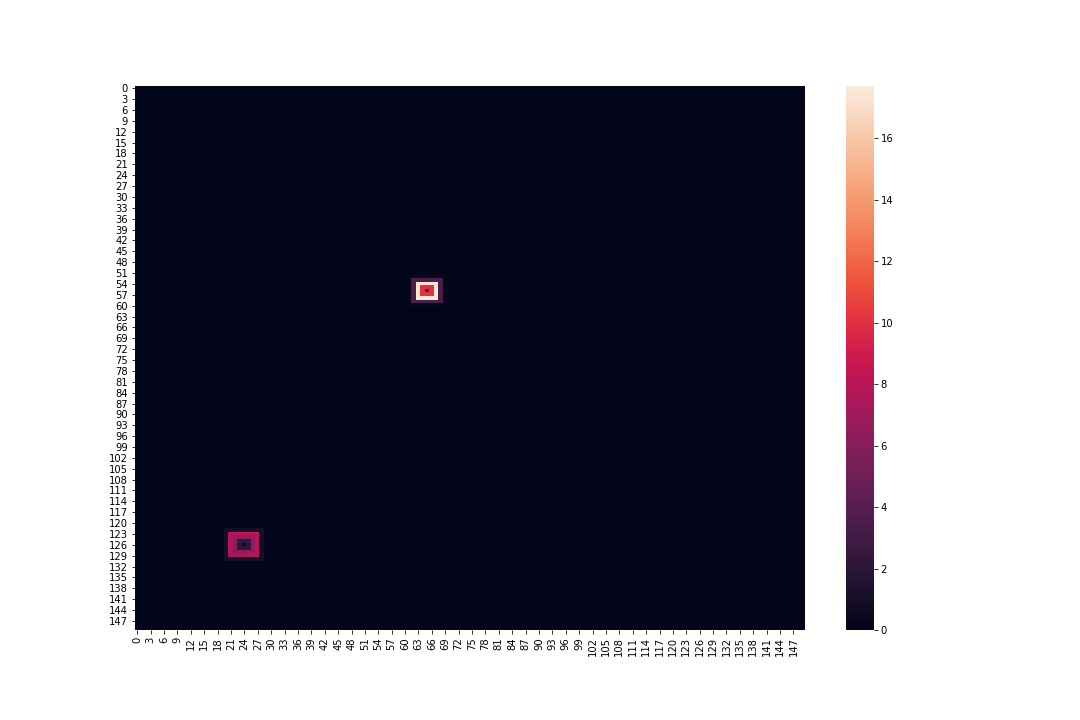
\includegraphics[scale=0.15]{../no_quarantine/no_quarantine_heatmap_3.png}
  \centering
  \caption{Simulating with BFS. Each image taken every 10 days over a
  40 day period.}
\end{figure}

\begin{figure}[ht]
  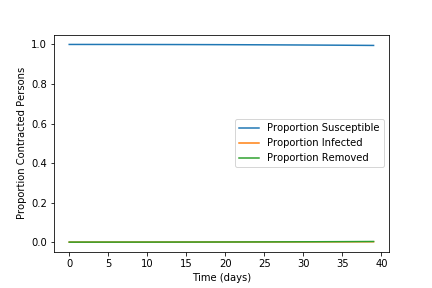
\includegraphics[scale=0.75]{../no_quarantine/no_quarantine_plt.png}
  \centering
  \caption{BFS spread. The plot of proportions of S, I, R over a 40 day period.}
  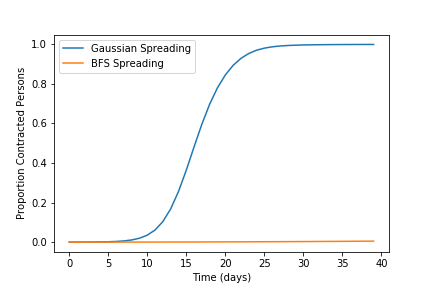
\includegraphics[scale=0.75]{../combined_spread.png}
  \centering
  \caption{A comparison in the total removed over time in each model.}
\end{figure}

\begin{center}
  \textbf{7. Conclusions and Recommendations}
\end{center}

From the results it is clear that mobility plays a critical factor in fueling a
pandemic. By reducing the amount of travel in an epidemic region, the spread of
the disease is reduced.

In January 2019, the WHO published a SEIR model specifically for COVID-19 in
Wuhan. The the new population `E' stands for Exposed, which means a susceptible
person has been exposed to the disease, but the not . It is an intermediary phase between susceptible and infected.


\end{document}
